\documentclass[11pt]{article}
\usepackage[utf8]{inputenc}
\usepackage[margin=1in]{geometry}
\usepackage{natbib}
\bibliographystyle{abbrvnat}
\usepackage{amsmath}
\usepackage{amssymb}
\usepackage{comment}
\usepackage{bbm}
\usepackage{amsthm}
\geometry{a4paper}
\usepackage{graphicx}
\usepackage{booktabs}
\usepackage{array}
\usepackage{paralist}
\usepackage{verbatim}
\usepackage{subfig}
\usepackage{multirow}
\usepackage{rotating}
\usepackage{fancyhdr}
\usepackage{hyperref}
\usepackage{bm}
\usepackage{xcolor}
\usepackage{listings}
\lstset{basicstyle=\ttfamily,
  showstringspaces=false,
  commentstyle=\color{red},
  keywordstyle=\color{blue}
}
\pagestyle{fancy}
\renewcommand{\headrulewidth}{0pt}
\lhead{}\chead{}\rhead{}
\lfoot{}\cfoot{\thepage}\rfoot{}
\usepackage{algorithm}
\usepackage{algpseudocode}
\usepackage{fancyvrb}
\usepackage{pythonhighlight}

\title{%
  Summer project \\
  \large Learning to bid above a threshold}
\date{May 2024}
\author{02344391}

\begin{document}

\maketitle

\paragraph*{Model 1}

\begin{itemize}
  \item Probability space $(\Omega, \mathcal{F}, \mathbb{P})$ with filtration $\mathbb{F} = (\mathcal{F}_t)_{t=1}^T$;
  \item Threshold $\tau_t$ is stationary: for each $t = 1, \dots T$, $\tau_t = \tau + \epsilon_t$, where $\tau$ is a constant
and $(\epsilon_t)_{t = 1}^T$ i.i.d with mean $0$ and variance $\sigma^2$;
  \item At each round $t$, we propose a bid: $b_t$;
  \item At each round $t$, we have the information: $\delta_t = \mathbb{I}_{\{\tau_t \leq b_t\}}$;
  \item Extension: after some delay $d$, we observe the true value. Thus for $t > d$, $\tau_{t-d}$ is $\mathcal{F}_t$- measurable.
\end{itemize}

The goal is to find a strategy that allows for bids above the threshold as quickly as possible while minimising the difference 
between the threshold and the bid. 
If we consider the model with the true threshold values provided with a delay, this information should be used to model the 
distribution of the thresholds, particularly to find the variance and provide a confidence interval that the bid is above the threshold.

We suppose that for any $t = 1, \dots T$, $\epsilon_t \sim \mathcal{N}(0, \sigma^2)$. In this initial model, we aim to write an algorithm that proposes bids to achieve a desired acceptance rate. Indeed, depending on the 
desired objectives, the strategies can vary: a high acceptance rate might correspond to high bids. In an auction example, this could 
lead to significant financial loss, and we might prefer a lower acceptance rate.

\subsection*{$\tau$ is known}

Initially, we assume that $\tau$ is known; the bids will then aim to find the value of $\sigma^2$.
We can, for example, consider the case of an auction where all items have the same price estimate $\tau$, but the price is noisy.

According to the model's assumptions, 
we have access to data that is right and left censored; indeed, $\delta_t$ indicates whether bid $b_t$ is above the threshold $\tau_t$ or not. In the case 
where we consider the threshold values known after a certain delay, we also have observed data. 
We use the Expectation Maximisation (EM) Algorithm to estimate the value of $\sigma^2$.
("Expectation-Maximization (EM) was described by Arthur Dempster, Nan Laird, and Donald Rubin in a classic 1977 paper in the Journal of the Royal Statistical Society.")

Observed data are denoted by $y = (y_i)_{i = 1}^N$ generated by $(Y_i)_{i = 1}^N$, and unobserved data are denoted by $\mathcal{T} = (\tau_i)_{i=1}^M$. We know that $Y_1, \dots Y_N$ and $\tau_1, \dots \tau_M$ are iid
$\sim \mathcal{N}(\tau, \sigma^2)$ where $\tau$ is known. We observe $\delta = (\delta)_{i=1}^M$:
$$
\delta_i= \left\{
    \begin{array}{ll}
        0 & \mbox{if } \tau_i > b_i \\
        1 & \mbox{otherwise.}
    \end{array}
\right., \quad i = 1, \dots M.
$$

Here, we have reindexed the bids and thresholds to separate the observed data from the unobserved data.

EM algorithm:
\paragraph*{"E-step":}
$$Q(\sigma, \sigma_n) = \mathbb{E}\left[\log(f(\mathcal{T},Y|\sigma))|Y = y, \delta, \sigma_n\right]$$
where $f$ is the density of the complete data.

We can derive $Q(\sigma, \sigma_n)$:
\begin{align*}
  Q(\sigma, \sigma_n) &= \mathbb{E}\left[\log(f(\mathcal{T},Y|\sigma))|Y = y, \delta, \sigma_n\right] \\
  &= - \frac{N}{2} \log(2 \pi \sigma^2) - \frac{1}{2\sigma^2} \sum_{i = 1}^N (y_i - \tau)^2 - \frac{M}{2}\log(2 \pi \sigma^2)  - \frac{1}{2\sigma^2} \sum_{i = 1}^M \mathbb{E}\left[(\tau_i - \tau)^2| \delta_i, \sigma_n\right]\\
  &= - \frac{N + M}{2} \log(2 \pi \sigma^2) - \frac{1}{2\sigma^2} \sum_{i = 1}^N (y_i - \tau)^2 - \frac{1}{2\sigma^2} \sum_{i = 1}^M \mathbb{E}\left[(\tau_i - \tau)^2| \delta_i, \sigma_n\right]
\end{align*}

We need to compute $\mathbb{E}\left[(\tau_i - \tau)^2| \delta_i, \sigma_n\right]$ for $i = 1, \dots M$. Let $i \in \{1, \dots,  M\}$, we suppose $\delta_i = 1$, thus $\tau_i \leq b_i$. Then:
\[
\mathbb{E}\left[(\tau_i - \tau)^2| \delta_i, \sigma_n\right] = \frac{1}{\mathbb{P}[\tau_i \leq b_i | \sigma_n]}\mathbb{E}\left[ (\tau_i - \tau)^2 \mathbb{I}_{\{\tau_i \leq b_i\}}|\sigma_n\right]
\]
First, since $\tau_i | \sigma_n \sim \mathcal{N}(\tau, \sigma_n^2)$,
$$ \mathbb{P}[\tau_i \leq b_i | \sigma_n] = \mathbb{P}\left[\left.\frac{\tau_i - \tau}{\sigma_n} \leq \frac{b_i - \tau}{\sigma_n} \right| \sigma_n\right] = \Phi\left(\frac{b_i - \tau}{\sigma_n}\right)$$
where $\Phi$ is the CDF of the standard normal distribution.

Then,
\begin{align*}
  \mathbb{E}\left[(\tau_i - \tau)^2 \mathbb{I}_{\{\tau_i \leq b_i\}}|\sigma_n\right] &= \int_{-\infty}^{b_i}\frac{(t-\tau)^2}{\sqrt{2\pi \sigma_n^2}}\exp\left(-\frac{1}{2\sigma_n^2}(t - \tau)^2\right)dt\\
  & = \sigma_n^2 \int_{-\infty}^{b_i}\frac{(t-\tau)^2}{\sigma_n^2}\frac{1}{\sqrt{2\pi}}\exp\left(-\frac{1}{2\sigma_n^2}(t - \tau)^2\right)\frac{dt}{\sigma_n}\\
  & = \sigma_n^2 \int_{-\infty}^{\frac{b_i - \tau}{\sigma_n}} u^2 \frac{1}{\sqrt{2\pi}}\exp\left(-\frac{u^2}{2}\right)du
\end{align*}

The PDF of the standard normal distribution is denoted by $\phi$, and by integration by parts:
\begin{align*}
\int_{-\infty}^{\frac{b_i - \tau}{\sigma_n}} u^2 \frac{1}{\sqrt{2\pi}}\exp\left(-\frac{u^2}{2}\right)du & = \left[- u \phi(u)\right]_{-\infty}^{\frac{b_i - \tau}{\sigma_n}} + \int_{-\infty}^{\frac{b_i - \tau}{\sigma_n}} \phi(u)du\\
& = -\frac{b_i - \tau}{\sigma_n} \phi\left(\frac{b_i - \tau}{\sigma_n}\right) + \Phi\left(\frac{b_i - \tau}{\sigma_n}\right)
\end{align*}

Finally:

\[
  \mathbb{E}\left[(\tau_i - \tau)^2| \delta_i, \sigma_n\right] = \sigma_n^2 \left(1 - \frac{b_i - \tau}{\sigma_n} \frac{\phi\left(\frac{b_i - \tau}{\sigma_n}\right)}{ \Phi\left(\frac{b_i - \tau}{\sigma_n}\right)}\right).
\]

In a similar way, if $\delta_i = 0$:

\[
  \mathbb{E}\left[(\tau_i - \tau)^2| \delta_i, \sigma_n\right] = \sigma_n^2 \left(1 + \frac{b_i - \tau}{\sigma_n} \frac{\phi\left(\frac{b_i - \tau}{\sigma_n}\right)}{ 1 - \Phi\left(\frac{b_i - \tau}{\sigma_n}\right)}\right).
\]

We deduce:
\begin{align*}
  Q(\sigma, \sigma_n) &= - \frac{N + M}{2} \log(2 \pi \sigma^2) \\
  &- \frac{1}{2\sigma^2} \sum_{i = 1}^N (y_i - \tau)^2 \\
  &- \frac{\sigma_n^2}{2\sigma^2} \sum_{i = 1}^M \left[ \left(1 - \frac{b_i - \tau}{\sigma_n} \frac{\phi\left(\frac{b_i - \tau}{\sigma_n}\right)}{ \Phi\left(\frac{b_i - \tau}{\sigma_n}\right)}\right)\delta_i +  \left(1 + \frac{b_i - \tau}{\sigma_n} \frac{\phi\left(\frac{b_i - \tau}{\sigma_n}\right)}{ 1 - \Phi\left(\frac{b_i - \tau}{\sigma_n}\right)}\right)(1-\delta_i)\right]
\end{align*}

\paragraph*{"M-step":}
We compute $\frac{\partial Q(\sigma, \sigma_n)}{\partial \sigma^2}$:

\begin{align*}
  \frac{\partial Q(\sigma, \sigma_n)}{\partial \sigma^2} &= - \frac{N + M}{2 \sigma^2} \\
  &+ \frac{1}{2\sigma^4} \sum_{i = 1}^N (y_i - \tau)^2 \\
  &+ \frac{\sigma_n^2}{2\sigma^4} \sum_{i = 1}^M \left[ \left(1 - \frac{b_i - \tau}{\sigma_n} \frac{\phi\left(\frac{b_i - \tau}{\sigma_n}\right)}{ \Phi\left(\frac{b_i - \tau}{\sigma_n}\right)}\right)\delta_i +  \left(1 + \frac{b_i - \tau}{\sigma_n} \frac{\phi\left(\frac{b_i - \tau}{\sigma_n}\right)}{ 1 - \Phi\left(\frac{b_i - \tau}{\sigma_n}\right)}\right)(1-\delta_i)\right]
\end{align*}

And $Q(\sigma, \sigma_n)$ is maximised for:
\[
  {\sigma^*}^2 = \frac{1}{N + M} \left[ \sum_{j = 1}^N (y_j - \tau)^2 + \sum_{i = 1}^M \left(1 - \tilde{b}_i^{(n)} \frac{\phi\left(\tilde{b}_i^{(n)}\right)}{ \Phi\left(\tilde{b}_i^{(n)}\right)}\right)\delta_i +  \left(1 + \tilde{b}_i^{(n)} \frac{\phi\left(\tilde{b}_i^{(n)}\right)}{ 1 - \Phi\left(\tilde{b}_i^{(n)}\right)}\right)(1-\delta_i)\right]
\]
where $\tilde{b}_i^{(n)} = \frac{b_i - \tau}{\sigma_n}$.

\subsection*{$\tau$ is unknown}

Now we suppose $\tau$ and $\sigma^2$ are unknown. In a similar way:
\paragraph*{"E-step":} we compute $Q((\tau, \sigma), (\tau_n, \sigma_n))$, thus, we consider:
\[
  \mathbb{E}\left[(\tau_i - \tau)^2| \delta_i, \tau_n, \sigma_n \right] = \mathbb{E}\left[\tau_i^2 | \delta_i, \tau_n, \sigma_n \right] - 2 \tau \mathbb{E}\left[\tau_i| \delta_i, \tau_n, \sigma_n \right] + \tau^2.
\]

Now:
\[ 
\tilde{b}_i^{(n)} =  \frac{b_i - \tau_n}{\sigma_n}.
\]
\paragraph*{(i)} $\mathbb{E}\left[\tau_i^2 | \delta_i, \tau_n, \sigma_n \right]$


If $\delta_i = 1$:

\begin{align*}
  \mathbb{E}\left[\tau_i^2 | \delta_i, \tau_n, \sigma_n \right] & = \frac{1}{\Phi\left(\tilde{b}_i^{(n)}\right)} \int_{- \infty}^{b_i}\frac{x^2}{\sqrt{2 \pi}\sigma_n}\exp\left(-\frac{(x-\tau_n)^2}{2 \sigma_n^2}\right) dx \\
  & = \frac{1}{\Phi\left(\tilde{b}_i^{(n)}\right)} \int_{- \infty}^{\tilde{b}_i^{(n)}}(\sigma_n u + \tau_n)^2\exp\left(\frac{-u^2}{2}\right) du \\
  & = \frac{1}{\Phi\left(\tilde{b}_i^{(n)}\right)} \left(\sigma_n^2 \int_{-\infty}^{\tilde{b}_i^{(n)}} u^2 \phi(u)du + 2\sigma_n \tau_n \int_{-\infty}^{\tilde{b}_i^{(n)}} u \phi(u)du + \tau_n^2 \int_{-\infty}^{\tilde{b}_i^{(n)}} \phi(u)du \right).
\end{align*}

We find:
\[
  \sigma_n^2 \int_{-\infty}^{\tilde{b}_i^{(n)}} u^2 \phi(u)du = \sigma_n^2 \left( \Phi\left(\tilde{b}_i^{(n)}\right) - \tilde{b}_i^{(n)} \phi\left(\tilde{b}_i^{(n)}\right)\right)
\]
\[
  2\sigma_n \tau_n \int_{-\infty}^{\tilde{b}_i^{(n)}} u \phi(u)du = - 2 \sigma_n \tau_n \phi\left(\tilde{b}_i^{(n)}\right)
\]
\[
  \tau_n^2 \int_{-\infty}^{\tilde{b}_i^{(n)}} \phi(u)du = \tau_n^2 \Phi\left(\tilde{b}_i^{(n)}\right)
\]

Therefore,
\[
  \mathbb{E}\left[\tau_i^2 | \delta_i, \tau_n, \sigma_n \right] = \sigma_n^2 + \tau_n^2 - \sigma_n (b_i + \tau_n) \frac{\phi\left(\tilde{b}_i^{(n)}\right)}{\Phi\left(\tilde{b}_i^{(n)}\right)}.
\]

And if $\delta_i = 0$:
\[
  \mathbb{E}\left[\tau_i^2 | \delta_i, \tau_n, \sigma_n \right] = \sigma_n^2 + \tau_n^2 + \sigma_n (b_i + \tau_n) \frac{\phi\left(\tilde{b}_i^{(n)}\right)}{1 - \Phi\left(\tilde{b}_i^{(n)}\right)}.
\]

\paragraph*{(ii)} $\mathbb{E}\left[\tau_i| \delta_i, \tau_n, \sigma_n \right]$

If $\delta_i = 1$ (similar):
\[
\mathbb{E}\left[\tau_i| \delta_i, \tau_n, \sigma_n \right] = \tau_n - \sigma_n \frac{\phi\left(\tilde{b}_i^{(n)}\right)}{\Phi\left(\tilde{b}_i^{(n)}\right)}
\]

If $\delta_i = 0$:
\[
\mathbb{E}\left[\tau_i| \delta_i, \tau_n, \sigma_n \right] = \tau_n + \sigma_n \frac{\phi\left(\tilde{b}_i^{(n)}\right)}{1 - \Phi\left(\tilde{b}_i^{(n)}\right)}
\]

\paragraph*{(iii)}
Finally:
\[
  \mathbb{E}\left[(\tau_i - \tau)^2| \delta_i, \tau_n, \sigma_n \right]= \left\{
    \begin{array}{ll}
      \sigma_n^2 + (\tau - \tau_n)^2 + \sigma_n (2 \tau - (b_i + \tau_n)) \frac{\phi\left(\tilde{b}_i^{(n)}\right)}{\Phi\left(\tilde{b}_i^{(n)}\right)}  & \mbox{if } \delta_i = 1 \\
      \sigma_n^2 + (\tau - \tau_n)^2 - \sigma_n (2 \tau - (b_i + \tau_n)) \frac{\phi\left(\tilde{b}_i^{(n)}\right)}{1 - \Phi\left(\tilde{b}_i^{(n)}\right)} & \mbox{otherwise.}
    \end{array}
\right..
\]

\paragraph*{"M-step":}
We compute $\frac{\partial Q((\tau, \sigma), (\tau_n, \sigma_n))}{\partial \tau}$:

\[
  \frac{\partial Q((\tau, \sigma), (\tau_n, \sigma_n))}{\partial \tau} = \frac{1}{\sigma^2}\left(\sum_{i=1}^N y_i - (M+N) \tau + \sum_{i=1}^M \mathbb{E}\left[\tau_i| \delta_i, \tau_n, \sigma_n \right]\right)
\]

And $\frac{\partial Q((\tau, \sigma), (\tau_n, \sigma_n))}{\partial \tau} = 0$ for:
\[
  \tau^* = \frac{1}{M+N}\left(\sum_{j=1}^N y_j + M \tau_n -  \sigma_n \sum_{i=1}^M  \left[\frac{\phi\left(\tilde{b}_i^{(n)}\right)}{\Phi\left(\tilde{b}_i^{(n)}\right)} \delta_i - \frac{\phi\left(\tilde{b}_i^{(n)}\right)}{1 - \Phi\left(\tilde{b}_i^{(n)}\right)} (1-\delta_i)\right] \right).
\]

Now we compute $\frac{\partial Q((\tau, \sigma), (\tau_n, \sigma_n))}{\partial \sigma^2}$:

\[
  \frac{\partial Q((\tau, \sigma), (\tau_n, \sigma_n))}{\partial \sigma^2} = - \frac{N + M}{2} \frac{1}{\sigma^2} + \frac{1}{2\sigma^4} \left(\sum_{i = 1}^N (y_i - \tau)^2 + \sum_{i = 1}^M \mathbb{E}\left[(\tau_i - \tau)^2| \delta_i, \sigma_n\right]\right)
\]

We deduce $Q((\tau, \sigma), (\tau_n, \sigma_n))$ is maximised for $\tau = \tau^*$ and:
\begin{align*}
  {\sigma^*}^2 &= \frac{1}{N + M}\left[ \sum_{j=1}^N(y_j - \tau^*)^2 + M (\sigma_n^2 + (\tau^* - \tau_n)^2)\right.\\
               &\left.+ \sigma_n \sum_{i=1}^M   (2 \tau^* - (b_i + \tau_n)) \frac{\phi\left(\tilde{b}_i^{(n)}\right)}{\Phi\left(\tilde{b}_i^{(n)}\right)} \delta_i  - (2 \tau^* - (b_i + \tau_n)) \frac{\phi\left(\tilde{b}_i^{(n)}\right)}{1 - \Phi\left(\tilde{b}_i^{(n)}\right)} (1 - \delta_i)\right]
\end{align*}

\section*{Bandits}

We assume that the threshold values are bounded and that the bounds are known $(b_{\inf}, b_{\sup})$. We partition the domain of the threshold values into different zones where $J$ arms can propose their bids. At time $t$, arm $J_t \in \{1, \dots J\}$ proposes a bid.

% \begin{figure}[H]
%   \centering
%   \includegraphics[height=7cm]{"../../figures/arms_thresholds.png"}
%   \caption{Partitioning of zones for each arm.}
%   \label{fig:partition_arm}
% \end{figure}
% \begin{figure}[H]
%   \centering
%   \includegraphics[height=7cm]{"../../figures/arms_zones_thresholds.png"}
%   \caption{Zones for each arm.}
%   \label{fig:zones_arm}
% \end{figure}

(Lecture notes)
"For any arm j, let
\[
 N_j(t) = \sum_{s=1}^{t} \mathbb{I}_{\{J_s = j\}}
\]
be the number of times arm $j$ has been played up to (and including) round $t$."

Now, we need to define the rewards for each proposed bid:
\[
  X_{j,t} = \delta_t (b_{\sup} - b_t)
\]

Here, the reward is higher if the bid is low; we aim to exceed the threshold 
with a minimised bid. However, if the bid is below the threshold, it is considered a failure, so the reward is 0.

We can define the empirical average reward of each arm as
\[
\hat{\mu}_{j,t} = \frac{1}{N_j(t)}\sum_{s=1}^{t} X_{j,s} \mathbb{I}_{\{J_s = j\}}.
\]

(Lecture notes)
"Lemma 3.2.1. (Hoeffding's Lemma) If the random variable $X$ takes values in $[a, b]$,
then $X$ is $\frac{b-a}{2}$ sub-Gaussian.

The regret of an algorithm, $\pi$, that plays actions $J_1, \dots, J_T$ over
$T$ rounds is defined as
\[
  \mathfrak{R}_T(\pi) = \sum_{t=1}^{T}(\mu^* - \mu_{J_t}) 
\]

where $\mu^* =  \max_{1\leq j \leq J} \mu_j$ and $\mu_{j}$ is the expected reward of arm $j$.

"

We suppose that arm $j$ proposes a bid in $[a_0, a_1]$ ($0\leq a_0 < a_1 \leq 1)$ uniformly and the threshold distribution is $\mathcal{N}(\tau, \sigma^2)$ (indendent of arm $j$). We compute
\[
\mu_j = \mathbb{E}[X_{j,t}] =  \mathbb{E}[\mathbb{I}_{\{\tau_t \leq b^{(j)}\}}(b_{\sup}-b^{(j)})]
\]
where $b^{(j)} \sim U[a_0, a_1]$ and $\tau_t \sim \mathcal{N}(\tau, \sigma^2)$.

We have:

\begin{align*}
  \mu_j &= \int_{-\infty}^{\infty}\int_{-\infty}^{\infty} \mathbb{I}_{\{x \leq b\}}(b_{\sup}-b) \frac{\phi(\frac{x - \tau}{\sigma})}{\sigma}\frac{\mathbb{I}_{\{a_0 \leq b \leq a_1\}}}{a_1 - a_0} dx db \\
  & = \frac{1}{a_1 - a_0}\int_{a_0}^{a_1}\int_{-\infty}^{b} (b_{\sup}-b) \frac{\phi\left(\frac{x - \tau}{\sigma}\right)}{\sigma} dx db \\
  & = \frac{1}{a_1 - a_0}\int_{a_0}^{a_1} (b_{\sup}-b) \int_{-\infty}^{b} \frac{\phi\left(\frac{x - \tau}{\sigma}\right)}{\sigma} dx db \\
  & = \left[- \frac{(b_{\sup}-b)^2}{2 (a_1 - a_0)} \Phi\left(\frac{b - \tau}{\sigma}\right) \right]_{a_0}^{a_1} + \frac{1}{a_1 - a_0}\int_{a_0}^{a_1}  \frac{(b_{\sup}-b)^2}{2 \sigma} \phi\left(\frac{b - \tau}{\sigma}\right)db.
\end{align*}

And (with $\tilde{a}_0 = \frac{a_{0} - \tau}{\sigma} $ and $\tilde{a}_1 = \frac{a_{1} - \tau}{\sigma}$):
\begin{align*}
  \int_{a_0}^{a_1}  \frac{(b_{\sup}-b)^2}{2 \sigma} \phi\left(\frac{b - \tau}{\sigma}\right)db & = \int_{\tilde{a}_0}^{\tilde{a}_1}  \frac{(b_{\sup}- \sigma b - \tau)^2}{2} \phi\left(b\right)db \\
  & = \frac{1}{2}\left(\sigma^2\int_{\tilde{a}_0}^{\tilde{a}_1} b^2 \phi\left(b\right)db\right. \\
  & + 2 \sigma (\tau - b_{\sup})\int_{\tilde{a}_0}^{\tilde{a}_1} b \phi\left(b\right)db \\
  & + \left.(\tau - b_{\sup})^2 \int_{\tilde{a}_0}^{\tilde{a}_1} \phi\left(b\right)db \right).
\end{align*}

We have:
\begin{align*}
  &\sigma^2 \int_{\tilde{a}_0}^{\tilde{a}_1} b^2 \phi(b)db = \sigma^2 \left( \Phi\left(\tilde{a}_1\right) -  \Phi\left(\tilde{a}_0\right) - \tilde{a}_1 \phi\left(\tilde{a}_1\right) + \tilde{a}_0 \phi\left(\tilde{a}_0\right)\right)\\
  &2 \sigma (\tau - b_{\sup}) \int_{\tilde{a}_0}^{\tilde{a}_1} b \phi(b)db = 2 \sigma (b_{\sup} - \tau) \left( \phi\left(\tilde{a}_1\right) - \phi\left(\tilde{a}_0\right)\right)\\
  &(\tau - b_{\sup})^2 \int_{\tilde{a}_0}^{\tilde{a}_1} \phi(b)db = (\tau - b_{\sup})^2 \left(\Phi\left(\tilde{a}_1\right) - \Phi\left(\tilde{a}_0\right) \right).
\end{align*}

Finally:
\begin{align*}
  \mu_j = &\frac{\sigma}{2(a_1 - a_0)}\biggl( \Phi\left(\tilde{a}_1\right) \left( \sigma - \tilde{a}_1\left(\tau - 2 b_{\sup} + a_1 \right)\right) - \Phi\left(\tilde{a}_0\right) \left( \sigma - \tilde{a}_0 \left(\tau - 2 b_{\sup} + a_0 \right)\right)\\
        &+ \phi\left(\tilde{a}_1\right)\left(  2 ( b_{\sup} - \tau)-\sigma \tilde{a}_1\right) - \phi\left(\tilde{a}_0\right)\left(  2 ( b_{\sup} - \tau)- \sigma \tilde{a}_0\right)\biggr)
\end{align*}

\bigskip

Now, we compute the second moment:

\begin{align*}
  \mathbb{E}[X_{j,t}^2] &= \mathbb{E}[\mathbb{I}_{\{\tau_t \leq b^{(j)}\}}(b_{\sup}-b^{(j)})^2] \\
  & = \frac{1}{a_1 - a_0}\int_{a_0}^{a_1} (b_{\sup}-b)^2 \int_{-\infty}^{b} \frac{\phi\left(\frac{x - \tau}{\sigma}\right)}{\sigma} dx db \\
  & = \left[- \frac{(b_{\sup}-b)^3}{3 (a_1 - a_0)} \Phi\left(\frac{b - \tau}{\sigma}\right) \right]_{a_0}^{a_1} + \frac{1}{a_1 - a_0}\int_{a_0}^{a_1}  \frac{(b_{\sup}-b)^3}{3 \sigma} \phi\left(\frac{b - \tau}{\sigma}\right)db.
\end{align*}

And (with $\tilde{a}_0 = \frac{a_{0} - \tau}{\sigma} $ and $\tilde{a}_1 = \frac{a_{1} - \tau}{\sigma}$):
\begin{align*}
  \int_{a_0}^{a_1}  \frac{(b_{\sup}-b)^3}{3 \sigma} \phi\left(\frac{b - \tau}{\sigma}\right)db & = \int_{\tilde{a}_0}^{\tilde{a}_1}  \frac{(b_{\sup}- \sigma b - \tau)^3}{3} \phi\left(b\right)db \\
  & = \frac{1}{3}\left(- \sigma^3\int_{\tilde{a}_0}^{\tilde{a}_1} b^3 \phi\left(b\right)db\right. \\
  & + 3 \sigma^2 (b_{\sup}- \tau)\int_{\tilde{a}_0}^{\tilde{a}_1} b^2 \phi\left(b\right)db \\
  & - 3 \sigma (b_{\sup}- \tau)^2\int_{\tilde{a}_0}^{\tilde{a}_1} b \phi\left(b\right)db \\
  & + \left.(b_{\sup}- \tau)^3 \int_{\tilde{a}_0}^{\tilde{a}_1} \phi\left(b\right)db \right).
\end{align*}

First,
\begin{align*}
  \sigma^3\int_{\tilde{a}_0}^{\tilde{a}_1} b^3 \phi\left(b\right)db = \sigma^3 \left( \tilde{a}_0^2 \phi(\tilde{a}_0) -\tilde{a}_1^2 \phi(\tilde{a}_1) + 2 \int_{\tilde{a}_0}^{\tilde{a}_1} b \phi(b) db\right)
\end{align*}

Then we have:
\begin{align*}
  \mathbb{E}[X_{j,t}^2] &= \frac{1}{3(a_1 - a_0)}\biggl( (b_{\sup}-a_0)^3 \Phi\left(\tilde{a}_0\right) - (b_{\sup}-a_1)^3 \Phi\left(\tilde{a}_1\right)\\
 & + \sigma^3 \left( \tilde{a}_1^2 \phi(\tilde{a}_1) -\tilde{a}_0^2 \phi(\tilde{a}_0) + 2 \left( \phi\left(\tilde{a}_1\right) - \phi\left(\tilde{a}_0\right)\right) \right)\\
 & + 3 \sigma^2 (b_{\sup}- \tau) \left( \Phi\left(\tilde{a}_1\right) -  \Phi\left(\tilde{a}_0\right) - \tilde{a}_1 \phi\left(\tilde{a}_1\right) + \tilde{a}_0 \phi\left(\tilde{a}_0\right)\right)\\
 & + 3 \sigma (b_{\sup}- \tau)^2 \left( \phi\left(\tilde{a}_1\right) - \phi\left(\tilde{a}_0\right)\right)\\
 & +  (b_{\sup}- \tau)^3 \left(\Phi\left(\tilde{a}_1\right) - \Phi\left(\tilde{a}_0\right) \right)\biggr)\\
 & = \frac{1}{3(a_1 - a_0)}\biggl(\Phi\left(\tilde{a}_1\right) \left( (b_{\sup}- \tau)^3 +3 \sigma^2 (b_{\sup}- \tau) - (b_{\sup}-a_1)^3\right)\\
 & - \Phi\left(\tilde{a}_0\right) \left( (b_{\sup}- \tau)^3 +3 \sigma^2 (b_{\sup}- \tau) - (b_{\sup}-a_0)^3\right) \\
 & + \phi\left(\tilde{a}_1\right)\left( \sigma^3 \left(\tilde{a}_1^2 + 2 \right) + 3 \sigma (b_{\sup}- \tau)^2 - 3 \sigma^2 (b_{\sup}- \tau)\tilde{a}_1  \right) \\
 & - \phi\left(\tilde{a}_0\right)\left( \sigma^3 \left(\tilde{a}_0^2 + 2 \right) + 3 \sigma (b_{\sup}- \tau)^2 - 3 \sigma^2 (b_{\sup}- \tau)\tilde{a}_0  \right) \biggr)
\end{align*}

From Bernstein's inequality for $\alpha > 0$, since $\left|\hat{\mu}_{j,t} -\mu_j\right|\leq b_{sup}$, here $b_{sup} = 1$:

\begin{align*}
  \mathbb{P}\left[\left|\hat{\mu}_{j,t} -\mu_j\right| > \alpha \ \right] \leq 2 \exp\left(- \frac{N_j(t)\alpha^2}{2 \mathbb{V}[X_j] + \frac{2}{3} \alpha}\right)
\end{align*}

Corollary: since $\left|\hat{\mu}_{j,t} -\mu_j\right|\leq 1$, with probability $1 - \delta$:

\begin{align*}
  \left|\hat{\mu}_{j,t} -\mu_j\right|  \leq \sqrt{\frac{4 \mathbb{V}[X_j] \log \frac{2}{\delta}}{N_j(t)}} + \frac{4 \log\frac{2}{\delta}}{3N_j(t)}
\end{align*}

Now, we want to find $n_{\delta} \in \mathbb{N}$ such that $\left|\hat{\mu}_{j,t} -\mu_j\right| \leq \alpha$ with probability $1 - \delta$. We need to solve, for $z\in \mathbb{R}$:
\[
- \alpha z^2 + \sqrt{4 \mathbb{V}\left[X_j\right] \kappa} z + \frac{4}{3} \kappa = 0
\]
where $\kappa = \log\frac{2}{\delta}.$

The roots are:
\[
z_{\pm} = \frac{\sqrt{\mathbb{V}\left[X_j\right] \kappa} \pm \sqrt{\mathbb{V}\left[X_j\right]\kappa + \frac{4}{3}\alpha \kappa}}{ \alpha}
\]

Finally, we find:
\[
  n_{\delta} \geq \log\frac{2}{\delta} \left(\frac{\sqrt{\mathbb{V}\left[X_j\right] } + \sqrt{\mathbb{V}\left[X_j\right] + \frac{4}{3}\alpha }}{\alpha}\right)^2
\]

We need to find a way to choose $\alpha$. Given different $\sigma$, the expected rewards are plot in figure (\ref{fig:partition50}), for a partition of 50 increments.

\begin{figure}[H]
  \centering
  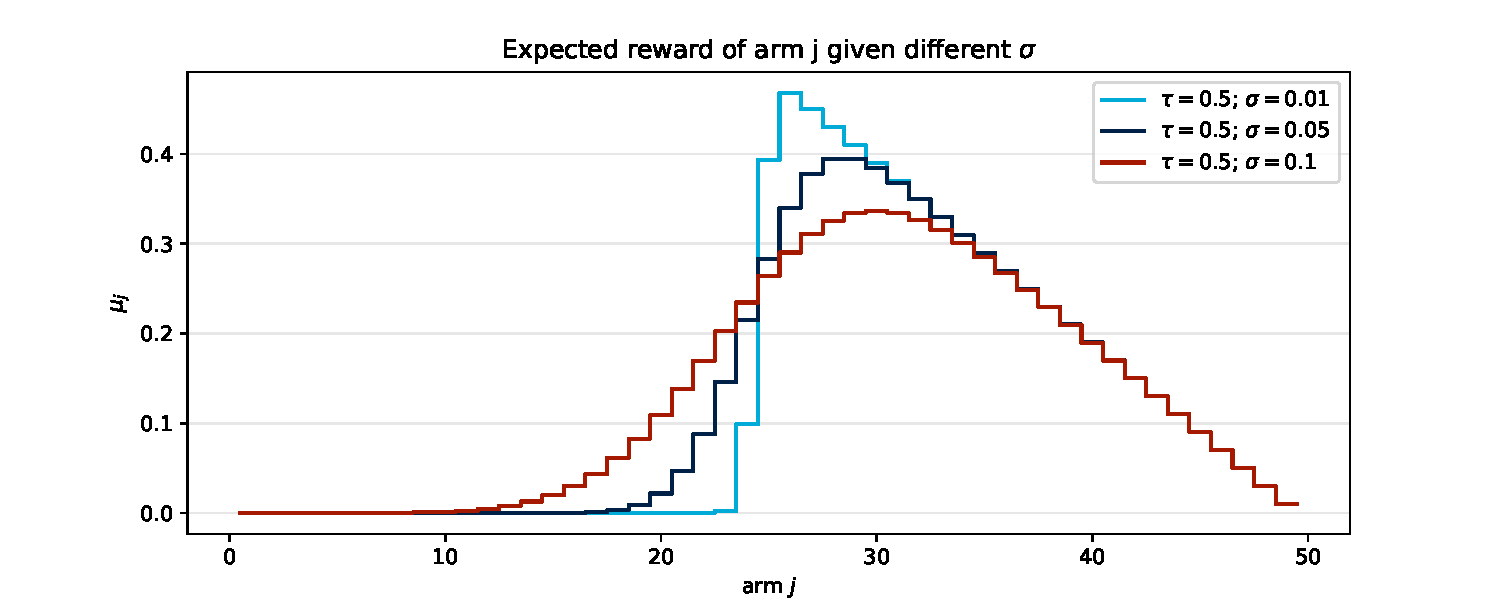
\includegraphics[height=6cm]{"../../figures/expect_rew_partition50.pdf"}
  \caption{Expected rewards for each arm (partition $[i/50, (i+1)/50], i = 0,\dots 49$)}
  \label{fig:partition50}
\end{figure}

When three arms are aligned, a rule is needed to definitively select the middle arm. 
In the algorithm used, the rule is simple: for a period of $n_{ep}$, the algorithm selects 
the middle arm with a probability $p$ and the other arms equally with a probability of $1 - p$. 
As long as the best arm is the middle one, the algorithm increases the probability $p$ until it tends towards 1.

\section{Last update}
\subsection*{Sequential halving Algorithm with EM}

\begin{itemize}
  \item Based on a predefined partition, run the sequential halving algorithm until 3 arms are aligned;
  \item Place bids on the three selected arms. If the empirical mean of the middle arm is not the largest, return to the sequential halving algorithm step;
  \item Otherwise, run the EM algorithm on these bids to obtain an estimate of the standard deviation ($\hat{\sigma}$) and the mean ($\hat{\tau}$) of the threshold distribution;
  \item Calculate the variance estimate for the middle arm using $\hat{\sigma}$ and $\hat{\tau}$, and calculate the estimate of half the difference between the mean of the best arm and that of the second best;
  \item Calculate the number of iterations ($n_{\text{Bernstein}}$) to construct a confidence interval according to Bernstein's inequality;
  \item Play the three selected arms $n_{\text{Bernstein}}$ times. If the middle arm is still the best, it is chosen; otherwise, return to the sequential halving algorithm step.
\end{itemize}

\section{Algorithms used so far}

In the simulations, $b_{\inf} = 0$ and $b_{\sup} = 1$

\begin{algorithm}[H]
  \caption{Naive epsilon-greedy algorithm}
  \label{code:epsilon_greedy}
  \begin{algorithmic}[0]
  \Require Number of zones $J$ (partition of $[b_{\inf}, b_{\sup}]$), vector of rewards $rew = \mathbf{0}_J$, counter $count = \mathbf{0}_J$, exploration rate $\epsilon$,
  vector of threshold $\tau$ of length $T$.
  \For{$ j = 1, \dots, J$} \Comment{Initialisation}
  \State Draw bid $b$ from a uniform distribution in zone $j$.
  \State Update $rew += reward(b, \tau_j)$; $count_j += 1$
  \EndFor
  \For{$ t = j+1, \dots, T$}
  \If{Uniform$([0,1]) < \epsilon$} \Comment{Exploration}
  \State Choose randomly $j^* \in \{1, \dots J\}$
  \Else \Comment{Exploitation}
  \State $j^* = \text{argmax}_{j \in \{1, \dots J\}} (rew_j / \max(1, count_j))_{j=1}^J$
  \EndIf
  \State Draw bid $b$ from a uniform distribution in zone $j^*$
  \State Update $rew_{j^*} += reward(b, \tau_t)$; $count_{j^*} += 1$
  \EndFor
  \State \Return $rew$, $count$
\end{algorithmic}
\end{algorithm}

\section{Time series}
refs:

"
Adapting to a Changing Environment: the Brownian Restless Bandits
Aleksandrs Slivkins
and Eli Upfal
"

$$\tau_t = \tau(t) + \epsilon_t$$ 
\newpage
%\bibliography{refs}
\end{document}